\documentclass[mscthesis]{usiinfthesis}
\usepackage{lipsum}
\usepackage{listings}

\lstdefinelanguage{algebra}
{morekeywords={import,sort,constructors,observers,transformers,axioms,if,
else,end},
sensitive=false,
morecomment=[l]{//s},
}

\title{A report on the decentralized web} %compulsory
\specialization{Specialization in Computer Systems}%optional
\subtitle{} %optional
\author{Eric Botter} %compulsory
\begin{committee}
\advisor{Prof.}{Fernando}{Pedone} %compulsory
\coadvisor{}{Leandro Pacheco}{De Sousa}{} %optional
\end{committee}
\Day{20} %compulsory
\Month{June} %compulsory
\Year{2018} %compulsory, put only the year
\place{Lugano} %compulsory

\dedication{} %optional
\openepigraph{Someone said \dots}{Someone} %optional

%\makeindex %optional, also comment out \theindex at the end

\begin{document}

\maketitle %generates the titlepage, this is FIXED

\frontmatter %generates the frontmatter, this is FIXED

\begin{abstract}
This is a very abstract abstract.

\lipsum
\end{abstract}

%\begin{abstract}[Zusammenfassung]
%optional, use only if your external advisor requires it in his/er language
%\end{abstract}

\begin{acknowledgements}
\lipsum
\end{acknowledgements}

\tableofcontents
%\listoffigures %optional
%\listoftables %optional

\mainmatter

\chapter{Introduction}\label{ch:intro}

The World Wide Web is probably the most popular and used service of the Internet, sometimes even confused with the Internet itself. It is very common nowadays to access the WWW (or most commonly known as simply ``the Web'') and browse websites from many platforms, from the typical desktop computer to the modern smartphone.

%TODO: give context about why a distributed web and what is happening at the moment

Let us define the scenario in which the Web lives. It is based on a client-server architecture, where Web servers provide objects (such as documents, images or files in general) to clients that request and display them, called \textit{user agents} (e.g. Web browsers).

In the Web, documents and objects are identified by a Uniform Resource Locator (URL), whose most important component is the domain name: it is a human-readable label that identifies a device within the Internet.
A domain name is composed by sequences of letters and symbols, separated by each other with dots. This separation is needed by the hierarchical structure of domain names, but we won't delve into the details of the Domain Name System here: we will talk more about it when we discuss naming, in Chapter \ref{ch:naming}.

To access a website, the client has to know the domain name associated to that website. This is usually provided by the user or by services such as search engines. The domain name is resolved to an IP address by using the Domain Name System.
Once obtained, the client opens a TCP connection towards that address on port 80, and starts exchanging messages using the HyperText Transfer Protocol (HTTP). %TODO - mention HTTPS

HTTP is a client-server, request-response protocol. Clients specify the details of the needed resource in the request and the server replies with the content or an error status if something went wrong (e.g. 404 Not Found). We won't explore HTTP as none of the projects that we will see rely on HTTP or any of its properties. %TODO explore HTTP? maybe expand on it as needed

There are different ways to setup a website. A content creator can either setup a custom server and upload a website there, or it can rent a server (either physical or virtual) from an existing provider.

\section{Problems in the current web} \label{sec:problems}
The main problem in the current Web is vulnerability to \textbf{censorship}. Since we have a direct relationship from domain names to websites (or from IP addresses to websites), it is relatively easy for powerful parties (including governments and ISPs) to block communications from users to a certain service. 
The main attacks that can be used to prevent communication towards a website are:
\begin{itemize}
	\item Denial of Service (DoS): a large volume of requests is sent towards the targeted server, which quickly runs out of available resources (such as bandwidth, simultaneously open connections, memory or CPU). Requests can be sent from a single device, but in current days requests are typically sent from multiple sources, in order to both increase the volume of traffic and make it difficult to identify and stop the origin of the attack: this is known as Distributed Denial of Service (DDoS).
	\item IP address blocking: packets towards a given address or address range are blocked. This attack can be enacted by routers that exchange packets regarding the targeted IP address, which can interrupt forwarding of said packets thus preventing any sort of communication, making the server effectively disconnected from the Internet.
	\item DNS hijacking: by altering DNS resolutions, the domain of the targeted website can either be deleted or edited to make it refer to another IP address, thus preventing access to the original content. This attack can be carried out by both the owners of the DNS resolver (by directly editing their records), or by third parties through an attack called DNS cache poisoning: an attacker pretending to be a valid name server intercepts DNS requests from other name servers and provides fake responses to alter the address of the targeted domain, also setting a high time-to-live so that the redirection is active for as long as possible. Another vector for DNS hijacking, though unrelated to DNS itself, is to remotely edit the configuration of typical home routers through known vulnerabilities, changing the DNS resolver to a malicious one.
\end{itemize}

We also have a problem of \textbf{trust}. When you access a website, there is no guarantee that the data you received is from the content creator, because HTTP is vulnerable to man-in-the-middle attacks. There is no mechanism to verify the authenticity of the transmitted data and the protocol does not use encryption, so anyone can forge a valid HTTP communication (even based on an ongoing one) and send it through the wires. We expand on this in Chapter \ref{ch:background}.

HTTPS resolves this issue by asymmetrically encrypting the communication channel, and authenticating the data that is sent, but the current trust system (X.509) is based on certificate authorities and is considered weak, which might allow for identity theft. %TODO - expand on this

Another important issue is \textbf{privacy} and handling of personal information: with the current scenario, whenever you connect to a website, that website privately stores data about you.
This data can be either automatically collected from user interactions, or can be provided directly by the user: consider, as an example, a social network, where users provide personal information such as their generalities, and the website collects data such as post interactions, number and timestamps of logins, and so on.
This effectively moves ownership of the data from the user to the company. Data that intrinsically belongs to the user (especially personal information such as name, address and phone number) are stored privately into the company server, and the user has limited control over it, since the only possible actions on the data are the ones defined by the company or required by law.

\section{Thesis structure}
This thesis has been structured as follows. The first chapter describes the Web in its current state and defines the open issues in its regard. The second chapter introduces some common definitions and describes the models used to analyze the Web and any of the projects that will subsequently be looked at; we also define the characteristics of the Distributed Web. The third chapter describes and analyses some projects that focus on distributing storage.
%TODO: summary of what we're going to do

\section{Thesis goals}
%todo

\chapter{Models and Definitions}
\label{ch:background}

We have to rethink the Web if we want to move it to a decentralized environment. The current Web is a centralized system: each website is owned by a party that we'll define as \textit{content creator}. The content creator owns the website and is responsible for distributing its content, either by using a self-owned and maintained web server or by publishing it to a dedicated service, known as \textit{web hosting} service provider (there are too many services currently online to present a somewhat accurate list of examples here). When using \textit{web server}, we will always refer to both these options, since in both cases there is always a web server that serves the website, whether it's owned by the content provider or by a company.
Although it's not required, the content creator usually also obtains a domain name to associate with the website.

This system is centralized because the website is accessible only through the web server. If obtained, the domain name will always direct towards that server (even if it changes its IP address, since that's one of the main purposes of DNS).

Let us introduce a very important concept in distributed systems: \textbf{failure}, and its related models.
We introduce it now to highlight the difference between a centralized environment and a decentralized (or distributed) one.

The failure model in which we could place the Web is a \textbf{stopping failure model}.
In this model, a process can \textbf{fail}, i.e. it stops functioning as intended, and the way a process fails is by stopping, or \textit{halting}. Once a process has halted, it remains in that state. Other processes are able to detect this failure, and the most common way that this is done is by giving a maximum response time to message exchanges with that process: if we expect a communication which does not happen within a time limit, we consider that process as failed (this is called detection by \textit{timeout}).

This means that we know that each entity will behave as expected, and in case of failure it will not function at all. In other words, we consider that entity as \textbf{trusted}, as it will never give a response which is not conforming to the protocol.

This model allows Web clients (browsers) %TODO - define them in the Introduction
and content creators to make certain assumptions on the behavior of web servers and other components:
\begin{itemize}
	\item Web clients assume that the content they request is returned without any modification;
	\item It is assumed that the channel through which the information is sent does not modify that data;
	\item Content creators assume that the website that they create is stored in the web server (and distributed) without any modification.
	%TODO - more?
\end{itemize}
In case of failure of the Web server, a browser will try to communicate with it, and after some time without receiving a response it will give up and show to the user an error message, of which an example can be found in Figure \ref{fig:browsertimeoutexample}.
\begin{figure}[b]
	\centering
	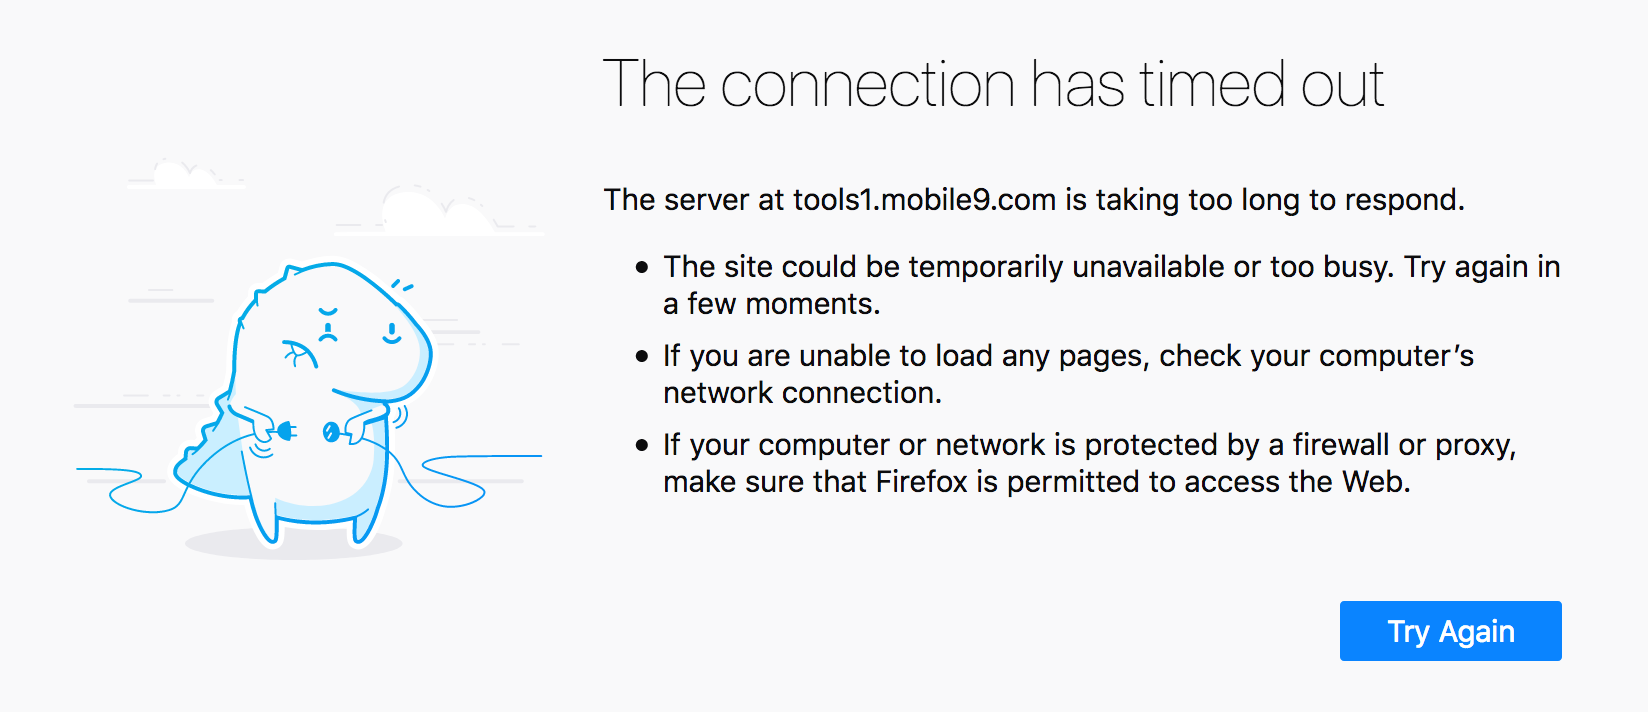
\includegraphics[width=0.9\linewidth]{img/browser-timeout-example}
	\caption{An error message for a connection timeout with a Web server given by Firefox 60.}
	\label{fig:browsertimeoutexample}
\end{figure}

One could argue that this model does not accurately represent the reality. For example, if a malicious third party takes over the communication channel, gaining complete control over each byte that it transports\footnote{An example of such a third party are Internet Service Providers.}, it can interfere and change the data that is transmitted. This is transparent to both the clients and the web server, since there is no mechanism in place to ensure that the data is \textit{integral}\footnote{TCP provides data integrity against transmission errors, which are in the order of few bits per kilobyte, but this is too weak in this scenario, where the entire TCP packet can be rewritten to appear unaltered.} -- and rightfully so, given that the communication channel is assumed to not alter data arbitrarily. This is known as a \textit{man-in-the-middle} attack.

To allow this scenario in our model we need to weaken it, by removing assumptions on what the communication channel will do during failure. We now allow arbitrary behavior, which means that processes under this weaker model can produce any kind of message, whether it complies to the protocol or not: they can lie, omit information or do just about anything, which also includes stopping and behaving properly. This model is the \textbf{Byzantine failure model}.
This is particularly useful to model malicious intentions: since failed entities can perform arbitrary actions, it is particularly important to consider situations that can cause the most damage to the system. Once we protect against these actions (and all possible other scenarios), we are sure to protect the system from any attacker that takes over the entities that we consider to be Byzantine.

Let's now place the communication channel in this Byzantine failure model.
HTTPS, the more secure Web protocol, is built around this weaker scenario. It introduces encryption and authentication of transmitted data, which allows it to be transferred over \textit{non-trusted} communication channels.
If the data is altered by a malicious third party during transmission, the client or the web server can detect it and react accordingly.

But what if we extend the Byzantine model to other entities? For example, if a content creator publishes a website on a web hosting service, that platform is technically able to delete or alter any file of that website, effectively sending to clients different information than the one intended by the author, and the clients would not notice this difference. HTTPS would not be able to protect against this attack, since it only protects the communication channel and not the website files themselves, which are encrypted by the web server only when transmitting them to a client: to do this, the web server has to access the files directly, and can therefore do whatever possible action to them, including editing and deleting them. Not only that: the web server is also able to send whatever content it desires (or refuse to serve content at all), since the client has no way of verifying that the content is as intended by its author.

What would we achieve if we protect the data itself from Byzantine attacks? If the data can be distributed by a non-trusted entity, then we don't need to rely on some specific and trusted system: \textit{anyone} can distribute it.

This effectively enables a \textbf{distributed Web}, where content is shared by a network of web servers that anyone can provide. We don't need to trust some hosting service provider with the website data, we can distribute our data to any of them and we will be sure that the information is going to be transmitted safely without modifications.

Let's see how this scenario can resolve the three problems described in Section \ref{sec:problems}:
\begin{itemize}
	\item \textbf{Censorship}: to allow web servers to expose Byzantine behavior means that any one of them can refuse to serve content. But note that we can't assume that every single web server fails with Byzantine consequences, just like we don't assume that in the current Web every single server will crash when contacted. We have to guarantee that some percentage of the servers will behave properly, without failing.\\
	This is why we need a \textbf{network} of web servers and not just one: that one server not only is exposed to all of the attacks mentioned in Section \ref{sec:problems}, but can also fail by refusing to serve content; if, instead of one, we have multiple web server (of which we are guaranteed that a percentage behaves properly), we know that if some web server fails (either on its own or by means of an attack) the rest of the network can still operate.

	\item \textbf{Trust}: by distrusting the web servers, we have made impossible for them to successfully send data different from what the content creator intended. Clients have a way to detect information manipulation and can discard such manipulated data.

	\item \textbf{Privacy} and handling of personal information: in a distributed environment, we no longer have websites that can privately store data about their users. This is because every website now is hosted on multiple servers: if they want to provide some form of consistency, they have to share or synchronize that data in some way. This would imply that the data is no longer private, but we cannot have public personal data available to multiple servers, especially when some of them have malicious intents.\\
	Among the different possibilities, we mention two options here: either the clients (and the clients only) store the private data, so that it is not shared in the network, or the data is uploaded in the network but in an encrypted way, so that only its owner can access it. We will see how different projects tackle this problem, and whether they solve it.
\end{itemize}

Many projects claim to implement the distributed Web. Every one of them provides a specific strength or focuses on a particular issue instead of building a complete, all-round system.
Unfortunately, such protocols are not well-known to the general public, and consequently are not widespread enough to be either standardized or integrated into modern state-of-the-art browsers.
But most importantly, creating such a protocol is very difficult.

Keep in mind that many of these projects do not define the model around which their platform is built. They mostly define the possible attacks and the related countermeasures they adopt. We will try to infer a model of the environment whenever we consider appropriate to do so, while trying stay as close to the project specifications as possible.

%\section{Challenges of creating a distributed Web}
%todo - But how exactly is it difficult to build the distributed Web? 

\chapter{Decentralizing Storage}

The first and most fundamental challenge in building the distributed Web is how to store the files that compose websites.

In the current Web, this is not generally a problem: you can either setup your own personal web server, exposed to the internet, that contains the website files, or you can upload those files to a web hosting service provider in order to serve them for you.
But now we have introduced a network of untrusted servers that are not necessarily going to distribute your files as you intended, if at all. How do we make sure that the files are still getting to the clients? How can clients be sure that they received the files exactly as their author has written them? To answer these two questions, each project has to implement two features, respectively.

The first one is an \textbf{incentive scheme}, i.e. a way to encourage nodes in a network to share data. If the incentive is strong enough, there will be more people that genuinely participate in the system, thus reducing the relative amount of intentional Byzantine behavior. Furthermore, if there is no incentive to share data, nodes will just obtain what they need and then leave the network, without contributing to other node's downloads, thus reducing the overall performance of the system, possibly even rendering it useless if this behavior is intentionally brought to the extreme (in other words, an attack is performed).

The second one is \textbf{data verification}: each system must provide a way to verify the integrity of the data that is transmitted. This is needed because everyone in the system can fail and transmit arbitrary data: who receives the data must be able to verify the received information, in order to detect and possibly discard it (maybe going as far as taking action w.r.t. the failed sender, for example by blocking communications). It usually involves cryptographic hashing, sometimes combined with asymmetric cryptography.

Another key component is a distributed storage system, but in general of any peer-to-peer network, is \textbf{peer discovery}, i.e. a mechanism through which a client can obtain a list of currently active peers that can be contacted. This is because on the Internet, it is impossible to find which devices are offering which services (especially if these devices keep moving and disconnecting all the time), without either knowing them directly, or looking them up using a dedicated directory that lists and keeps track of such devices. This directory can be either centralized or decentralized, and comparing the two options leads to the same advantages and disadvantages that we discussed previously. It would make sense to prefer a decentralized directory to a centralized one, but a completely distributed directory cannot exist, since it also needs to be discovered: a compromise has to be made. Often, projects with a distributed directory have a different process just to make the directory known to a client: this process is often referred to as \textit{peer discovery bootstrap}.
%todo - the above is probably confusing

%todo - define use cases to describe project functionalities? Like download a file, upload a file, etc.

\section{BitTorrent}\label{proj:bittorrent}

BitTorrent is probably the most known and used peer-to-peer file-sharing protocol. We take a look at BitTorrent both because of its popularity and because it is at the basis of ZeroNet, another project discussed in Section \ref{proj:zeronet}.

\subsection{Protocol overview}

Let us start with some definitions related to the BitTorrent protocol. A collection of files is known as a \textbf{torrent}, and to make distribution easier, each file is split into \textbf{blocks} of equal size. A torrent is described in a dedicated file called, unsurprisingly, \textbf{torrent file} (they are also known as \textit{metainfo files}), which contains a list of the files contained in that torrent and the cryptographic hash of each block (using the SHA-1 algorithm), plus some metadata, such as the name of the torrent, the block size, etc.

A BitTorrent client connected to and participating in the network is called a \textbf{peer}. Peers communicate with each other when they are aware of the same torrent: that group of peers is called a \textbf{swarm}. When a peer has all the parts of a torrent and is sharing them with the rest of network, it is called a \textbf{seeder}, and the operation of sharing data is called \textit{seeding}.

In BitTorrent, torrents are distributed out-of-band. It is assumed that when a peer obtains a torrent file, that file is legitimate and as intended by the torrent creator. Usually, torrent files can be obtained from the Web, often from dedicated websites and forums where users can upload their own torrent files: the documentation of BitTorrent only mentions the Web as a way to obtain torrent files.

To perform peer discovery, BitTorrent relies on \textbf{trackers}, dedicated servers that keep track of swarms for different torrents. Each torrent file lists the trackers that peers should contact (by announcing themselves) for that particular torrent. Although different torrents can rely on different (and multiple) trackers, this is a centralized peer discovery system: it is often the case that few trackers (in the order of tens) track the majority of torrents. If these trackers are shutdown or blocked, peers will have a hard time discovering each other. To counter this, BitTorrent later integrated two decentralized discovery mechanisms: DHT (which we cover in Appendix \ref{appx:dht}), and \textbf{Peer Exchange} (or PEX) that allows peers to trade information about their common swarm, so that each client can discover more peers, leading to a better connected swarm. Note that peers cannot join a swarm only through PEX: they have to first contact either a tracker or the DHT.

BitTorrent does not define how to bootstrap the connection to the DHT, leaving it as an implementation detail. Different clients employ different techniques, among which we can find the following:
\begin{itemize}
	\item Keep a long-lived cache of peers encountered: when the client is started, it tries to contact the peers in his cache to enter the DHT;
	\item Contact a known IP address/domain name that offers a dedicated DHT bootstrapping service;
	\item Retrieve an initial list of peers from a tracker, then access the DHT through them;
	\item Torrent files can contain information about nodes of the DHT or peers in the BitTorrent network.
\end{itemize}

To better describe the functionalities and mechanisms of BitTorrent, let's explore two fundamental scenarios: uploading a torrent into the network and downloading a torrent from the network.

To upload a torrent into the network, a user has to collect a set of files that will compose the torrent. By using a client that supports this functionality, the user can create a corresponding torrent file, which can then be distributed by the user on their preferred platform. The user's client now is aware of the torrent and has all its files: it is therefore seeding the torrent to other users.

To download a torrent from the network, a user has to obtain the torrent file first. The file is then passed to the client that will start to contact the swarm (through trackers, DHT or whichever system the torrent file specifies) and gather information about which peers have which data. It will then start downloading blocks from each peer, and will become a seeder when the download is complete.

BitTorrent's \textbf{incentive scheme} is well explained and analyzed by \cite{cohen2003incentives}, the creator of BitTorrent, and we will just summarize it here. It is based on a \textit{tit-for-tat} algorithm, and uses a mechanism known as \textbf{choking} to select the best peers for collaboration. Choking is refusal from a peer to share its blocks with another peer, who is said to be \textit{choked}; \textit{unchoking} is the opposite operation.

BitTorrent peers usually do not share data with all known downloading peers to reduce overhead of communications and best utilize the available bandwidth. Peers will start sending blocks to some other peer in the swarm, hoping that they return the favor and start sending data back. If the favor is not returned, the other peer is choked, and some other peer is chosen instead; otherwise, the peer will increase its bandwidth towards the other peer, and those peers will continue to share data between each other. This is done until a limit of simultaneously connected peers is reached, usually four but this is user-configurable. Every now and then, a peer will unchoke some random peer, hoping that a benevolent uploader is found: this is called an \textit{optimistic unchoke}, and it is done by replacing the worst-performing peer, which becomes choked. This allows to improve performance if the current transfers do not maximize a peer's bandwidth, but it can also degrade it if the new peer does not perform as good as the replaced one: this is why it is said to be \textit{optimistic}.

BitTorrent \textbf{data verification} system is based on cryptographic hashing, and is pretty straightforward: each torrent file contains the SHA-1 hash of every block in the torrent, so that peers can verify the integrity of each block upon downloading it.

\subsection{Analysis}

Let's try to infer the model in which BitTorrent is set. We have two main entities specific to the BitTorrent protocol: peers and trackers. 

We can safely place peers in a Byzantine failure model. This is because BitTorrent implements a data verification mechanism to ensure that the blocks received by the network are valid, by computing their hash and matching it with the one reported in the torrent file. It also discourages malicious activity by implementing a \textit{tit-for-tat}-like incentive scheme, of which we'll talk about later.

Identifying the failure model for the trackers is not so easy. This is because there is no method in place to ensure data validity: technically, a rouge tracker can omit data during communication with a peer or craft arbitrary responses, and a BitTorrent client would not notice this misbehavior. But what kind of damage can a Byzantine response from a tracker possibly cause? The simplest one is refusing to communicate, but this can also happen in a stopping failure model: a solution is to use data from another tracker (also note that clients can detect a missing response through timeout). A similar but more elaborate attack would be to provide a valid response, but without most if not all peers of the requested swarm: this is practically a denial of service attack, because a client would not be able to perform a download since it can't find any other peer to get the data from. To counter this attack, a client would have to lookup multiple trackers: it is often the case that a torrent file has references to more than one tracker, besides, a client can contact additional trackers than the ones specified in the torrent file, either automatically (a list of trackers that is added to torrents when starting the download process) or by user interaction. Lastly, a malicious tracker can include in a response fake peers that don't actually exist, that are currently unavailable or that only exhibit Byzantine behavior. Also this kind of attack falls under denial of service, since a client has to waste time contacting all these fake peers that will never respond correctly, if at all: a solution to this is, again, to combine data from multiple trackers.

Let's not forget that BitTorrent also has decentralized peer discovery methods, including a DHT. These systems, if available, will always be used alongside the tracker-based system, and since the DHT runs in a Byzantine failure model, we can consider it more reliable and trustworthy. Therefore, we can also place the trackers in a Byzantine model, since we won't be losing functionalities in doing so, although we might suffer from a performance perspective.

But there's still one element that needs consideration: the source of torrent files. The BitTorrent documentation (specifically in BEP 3) explicitly specifies that torrent files must be served over the Web, but this is not always the case, and it surely isn't enforced by BitTorrent clients: as long as they receive a torrent file, they will start to download the corresponding torrent. It is pretty clear that this source must be trusted, otherwise we would have an invalid torrent definition and the client would download data that is not what the torrent file or its source might suggest to be. %todo - expand on this? it seems pretty simple to me, maybe too much simple

So far the weakest link in this model is the source of the torrents. A user must find a reputable and trustworthy source from which torrents can be obtained. This is particularly an issue because of the controversial (and often illegal) content that can be obtained through the BitTorrent network: for example, malicious agents might setup websites which offer counterfeit software, while they actually distribute malware, or government agencies might take control of a popular torrent distribution website to track their users and alter or remove the torrent files that are offered (potentially affecting legitimate torrents).

But this is not the only issue in the network. Its incentive scheme has been thoroughly analyzed by the academic community and many publications demonstrate extensive research on the subject (we'll cite \cite{Zghaibeh2008}), outlining defects in the scheme and the possibility of downloading content without contributing to the network: this is known as \textbf{free riding}. \cite{locher2006free} describe a BitTorrent client named BitThief, that exploits optimistic unchokes to successfully download torrents while avoiding to share any resource, by always presenting itself as a new peer. Despite the presence of such behavior, the network is still functional and largely used today. The BitTorrent community has come up with \textit{etiquette} rules to maximize benign usage: for example, it is considered good practice to seed a torrent after downloading it, at least until the same amount of downloaded data has been uploaded (i.e. with a \textit{seed ratio} of 1: most clients will compute this value for the users).

%todo - continue? what can i write next?

\section{IPFS}\label{proj:ipfs}

The InterPlanetary FileSystem (IPFS for short) is a decentralized file system based on content-addressing coupled with a hypermedia distribution protocol. It has become popular as the \textit{Permanent Web}, as one of the goals of the project is ``to make the web faster, safer, and more open''.

\subsection{Protocol Description}



\subsection{Analysis}

\section{Ethereum Swarm}\label{proj:swarm}

\section{Filecoin}\label{proj:filecoin}

\section{Summary}

% todo - possible \chapter{Decentralizing logic}? This would just be Ethereum, and maybe Hashgraph

\chapter{Decentralizing Naming}\label{ch:naming}
%todo - start with DNS

\section{Namecoin}\label{proj:namecoin}

\section{Ethereum Name Service}\label{proj:ens}

\section{Analysis}


\chapter{Distributed Web Projects}

\section{ZeroNet}\label{proj:zeronet}

\section{Blockstack}\label{proj:blockstack}

\section{Analysis}


\chapter{Upcoming projects}

\section{Substratum}

\section{Hashgraph}


\chapter{Conclusions}

%As you can easily see from the above listing \citet{bbggs:iet07}
%define something weird based on the BPEL specification
%\citep{bpelspec}.
%\nocite{*}

\appendix 

\chapter{The Domain Name System - A brief overview}\label{appx:dns}
The Domain Name System is a decentralized naming system for devices connected to a network (including the Internet), currently defined with RFC 1034\cite{rfc:1034} and RFC 1035\cite{rfc:1035} and updated with successive RFCs throughout the years.

The DNS defines three components:
\begin{itemize}
	\item The \emph{domain name space} is a tree data structure, where nodes are identified by \emph{labels}: labels compose the domain names in a hierarchical way, by concatenation of labels separated by dots. For example, for the domain ``\texttt{www.example.com}'', ``\texttt{example.com}'' is a child of ``\texttt{com}'' and ``\texttt{www.example.com}'' is a child of ``\texttt{example.com}''.
	\item \emph{Name servers} are programs which store information about a subset of the domain space and references to other name servers which have information about the rest of the tree. Name servers have \emph{authority} over the parts of the tree of which they have complete information.
	\item \emph{Resolvers} are programs which receive queries from clients and respond with information extracted from the name servers. Resolvers only need to know directly just one name server to complete all possible queries: if that name server does not contain the requested information, the resolver uses its references to reach other name servers.
\end{itemize}
The domain name space has one root node, labeled with an empty string. Childs of this node are called \emph{top-level domains}, among which we can find ``\texttt{.com}'' and ``\texttt{.org}'', and two lettered \emph{country codes}, such as ``\texttt{.ch}'' and ``\texttt{.it}''. Currently, there are about one thousand different top-level domains\cite{website:tldlist}.

When resolving a hostname, resolvers query the root name server with the whole domain. The root name server usually replies with the address of the name server which has authority over the top-level domain of the hostname, but it also has facility to reply with the address of the actual server associated with the whole hostname. If the query has not been completed, the query is repeated with the correspondent top-level domain name server, and so on.

To reduce traffic towards the root name servers (and all other name servers), DNS resolvers implement a \emph{caching} system: results from name servers are stored for reuse, together with a time-to-live value specified from the name servers themselves. 

\chapter{Distributed Hash Table}\label{appx:dht}
%todo

\backmatter

\chapter{Glossary}
\begin{itemize}
	\item TCP
	\item ISP
	
\end{itemize}

%\bibliographystyle{alpha}
%\bibliographystyle{dcu}
\bibliographystyle{plainnat} %TODO - figure out how to work this
\bibliography{webrbiblio}

%\cleardoublepage
%\theindex %optional, use only if you have an index, must use
	  %\makeindex in the preamble
%\lipsum

\end{document}
